\documentclass[12pt]{article}
\usepackage[margin=1in]{geometry}
\usepackage{amssymb}
\usepackage{amsmath}
\usepackage{amsthm}
\usepackage{amsfonts}
\usepackage[shortlabels]{enumitem}
\usepackage{mathtools} 
\usepackage{amscd}        % For simple commutative diagrams
\usepackage{graphicx}
\usepackage{rotating}     % To rotate figures, tables, ...
\usepackage{color}
\usepackage{pdfpages}
\usepackage{blkarray, bigstrut, multirow}
\usepackage{hyperref}


\begin{document}
\begin{titlepage}
    \begin{center}
        \vspace*{1cm}

        \textbf{Winning with Arclight Phoenix}

        \vspace{0.5cm}
        The way of the Bird

        \vspace{1.5cm}

        \textbf{Josh Mulloy}

        \vspace{0.8cm}

        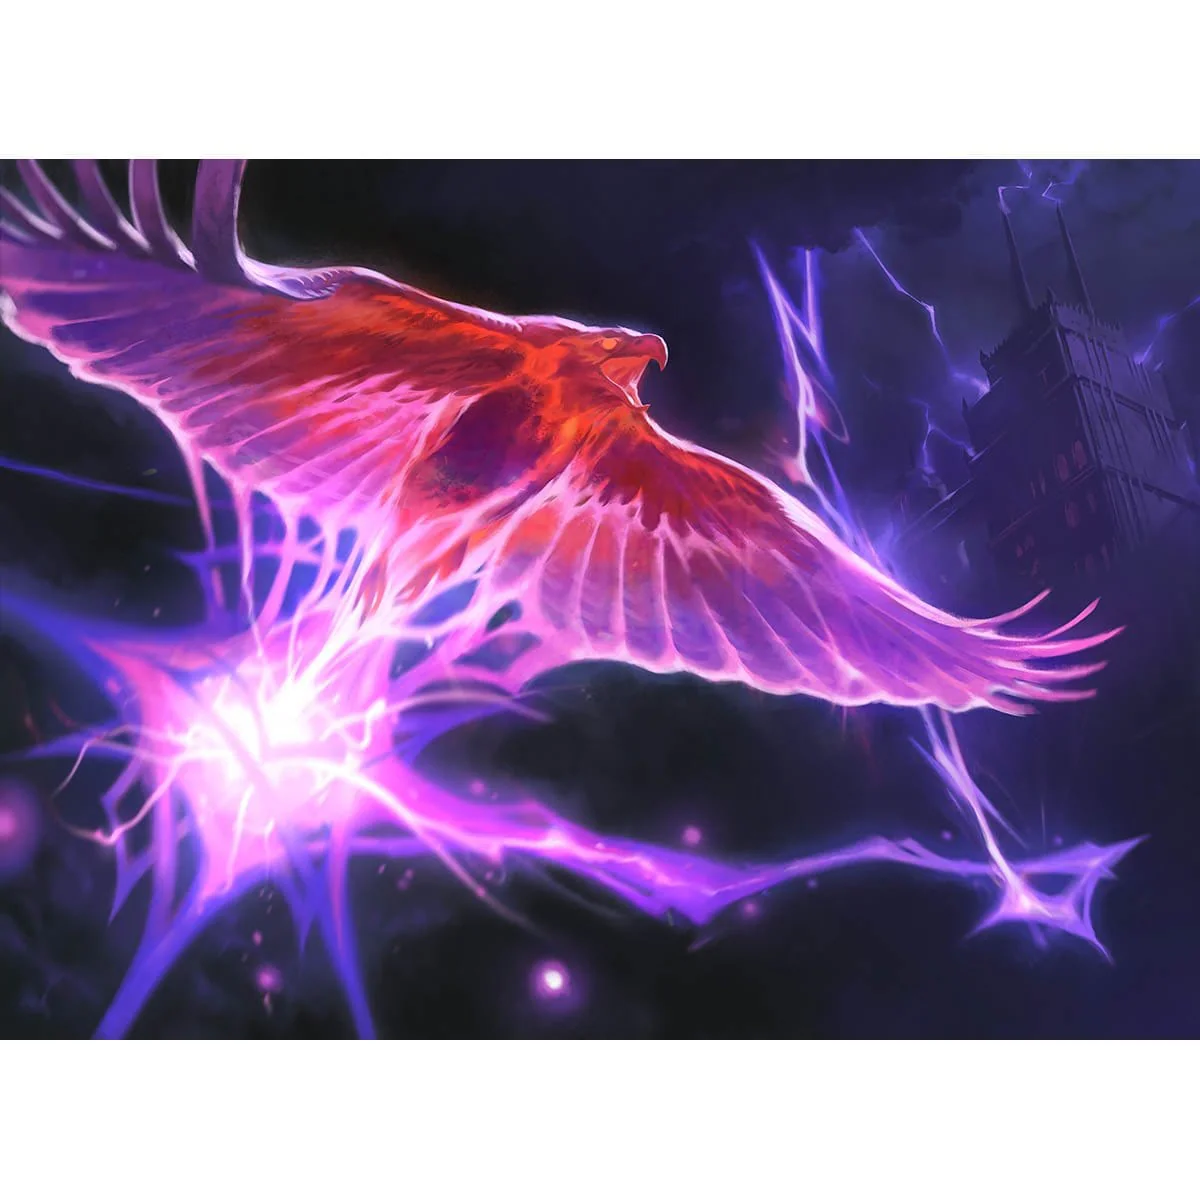
\includegraphics[width=0.7\textwidth]{arclight}

        \vfill

        A guide to playing arclight phoenix\\
        from a mid player
    \end{center}
\end{titlepage}

\tableofcontents

\clearpage
\section{Current List}
\begin{center}
    \href{https://www.mtggoldfish.com/deck/6561022#online}{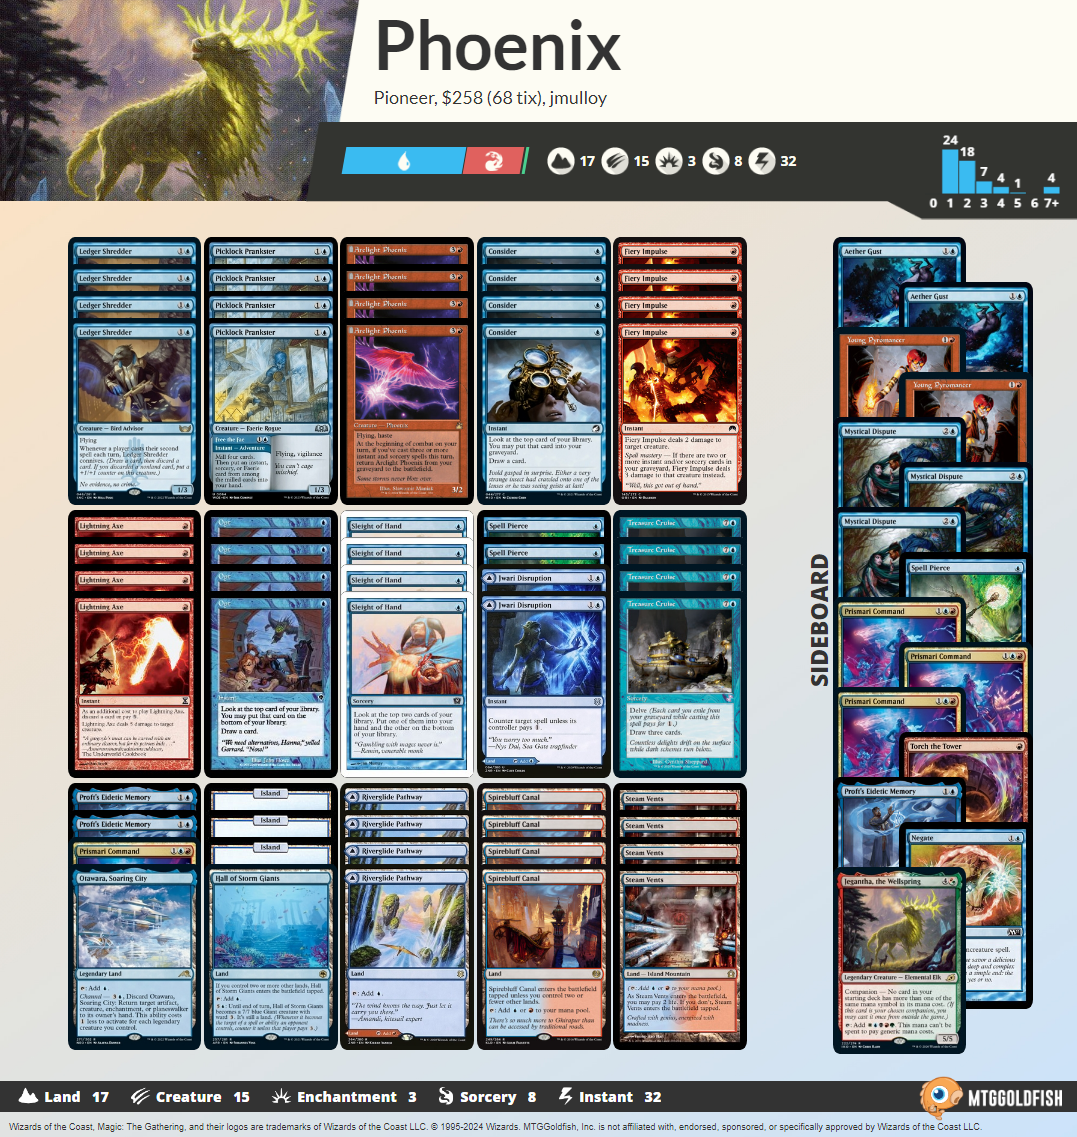
\includegraphics[width=1\textwidth]{decklist}}

    \href{https://www.mtggoldfish.com/deck/6561022}{https://www.mtggoldfish.com/deck/6561022}

    \vspace{0.5cm}

    \href{https://docs.google.com/spreadsheets/d/1DheUoGrQmpuwzbMDpPVJHcCrfe7UOyXSMSSkL8aXnv0/edit?usp=sharing}{Phoenix Matches (started tracking Aug 2024 [Challenge+ level]):}

    \href{https://docs.google.com/spreadsheets/d/1DheUoGrQmpuwzbMDpPVJHcCrfe7UOyXSMSSkL8aXnv0/edit?usp=sharing}{Spreadsheet Link}
\end{center}

\clearpage
\section{Why Phoenix?}
\subsection{Card Velocity}
Because phoenix plays 12 cantrips, 4 prankster, and 4 cruise, it is very easy to see most of your cards every game. This allows you to tune phoenix against basically any metagame, barring some pretty absurd things going on when phoenix is the clear best deck (like people registering waste not or lotus). Even when we are in one of these metas phoenix can still usually be tuned into a spot where we are fine into even these hate decks.

For example, with the newer prankster variants of phoenix we are able to play more spell pierce, depedning on the metagame. Some people even play a borrower in the main as a catch all that you can usually find when you need it. While I don't believe this to be better than just having Jegantha as a companion it speaks to how strong the ability to see so much of your deck is. This velocity is what makes the maindeck one ofs so interesting to me, something like maindeck primsari.

\subsection{Treasure Cruise}
I think a lot of people view phoenix as a deck that is just trying to put arclight phoenix into play as quickly as possible. While this is an admirable goal, it is not the main way that I play the deck. Often I would rather resolve a treasure crusie than put a single phoenix in play, and don't feel a strong urge to waste lightning axes because it will allow me to put phoenix into play.

I think if phoenix manages to get another card banned in the format, its going to be cruise. The fact that we can chain cruise to go from empty handed to a full grip in a single turn for only two mana means that often even if an opponent manages to get a little ahead they will need to kill us fast.

\subsection{Low vs. High Resource Games}
Phoenix as a deck is really good at playing games where it always has things to be doing with its mana. I call these games \emph{high resource games}. They are the games where we cantrip a lot, resolve a few cruises, and maybe have a shredder that goes unanswered for a few turns. It is really hard for us to lose these kinds of games. The deck is just so capable of finding all the answers we need while also putting a ton of pressure on in these games that most decks have to somehow prevent us from getting into one of these games. The low resource games are the ones where we are paying four mana for phoenix and 6 mana for lightning axe. They are the games where we don't find many cantrips and can't seem to find or maybe even cast a crusie.

Most of the games we lose are going to be games where we aren't able to get one of these high resource games going. This is what makes a lot of the hate so good into phoenix, but also what makes some of the hate less good than people think. Things like hearse, rip, and to a lesser extent leyline of the void are the main ways that decks try to keep us from creating high resource games. Leyline is specifically called out here because often we are able to turn a leyline game into a high resource game, or, if they don't have it in their opener, we can do enough to have a critical mass before they play it. The hate that is less good at stopping us in these spots are things like go blank, cling to dust, damping sphere, and grafdiggers cage. Just one of these cards isn't going to be enough to stop us, and in the case of cling, sphere, and cage I think these cards are just straight up bad into phoenix.

\subsection{It is Fun}
Phoenix is an interesting deck because you are able to see so many of your cards every game. You are going to have a ton of opporunities to make decisions, even if most of them don't matter, and that definitely makes it feel like you have more agency in the games than you do. For some reason I think this makes the game more fun for me. Furthermore, you just get to take a ton of game actions, and what are we playing magic for if not to take as many game actions as possible.

\vspace{0.4em}
\noindent I also just really like casting treasure cruise and attacking with 3/2s.

\clearpage
\section{The Details}
\subsection{Cantrip Sequencing}

\subsection{Playing Ledger Shredder}

\subsection{Thoughtseize}

\subsection{Graveyard Hate}

\subsection{Mulliganing}

\clearpage
\section{Card Choices}
\subsection{Main Deck Cards}
\label{sec:mainchoices}
\textbf{Jegantha:}
Much better than I expected it to be. Really good as just a card that can be put in hand to pitch to axe/shredder. Also fine as a beater in the low resource games.

\vspace{0.4em}
\noindent \textbf{Proft:}
Trespass plays pretty poorly with prankster, while this plays really well. Pretty sure this is just better in the mirror too. Definitely reduces our combo potential, making it a bit more important to chip in for damage when possible compared to the old phoenix lists, but you can still use this to kill people out of nowhere.

\vspace{0.4em}
\noindent \textbf{Cantrips:}
Seen lists playing 3 sleight, 4 opt, 4 consider. Do not do this if you want to win.

\vspace{0.4em}
\noindent \textbf{Spell Pierce:}
Very good against RB with game in the mirror and not dead against amalia. Kinda want to try going down to 2 and playing a md prismari.

\vspace{0.4em}
\noindent \textbf{Prismari Command:}
I feel very close to wanting one of these main, just haven't pulled the trigger yet. See SB section for why I like it.

\vspace{0.4em}
\noindent \textbf{Lands:}
The way I see it, phoenix lists have 4 flex slots for lands, usually choosing between 3rd island, hall of storm giants, jwari disruption, mountain, and stormcarved coast. I like jwari as something to bridge the gap to a turn 3 shredder that also gives us the ability to sometimes steal games by sniping something or making our opponent sequence weird. Hall is similar, where it is just there to shore up some games that we could be losing without it, specifically the low resource ones. I haven't felt a lot of pressure on red sources in my lists so I don't play an additional red source in mountain or stormcarved, but not playing them means you have to be a bit more careful deciding whether to put your pathways on red.

\vspace{0.4em}
\noindent \textbf{Torch the Tower:}
This card isn't better than impulse in basically any mu, including the mirror. I can't see myself ever playing one.

\subsection{Sideboard Cards}
\label{sec:sbchoices}
\noindent \textbf{Prismari Command:}
Does everything we want in the low resource games, while also dealing with most of the actually good hate against us. All 4 modes come up often. An important part of casting crusie in low resource post board games to pull ahead, acting as a quadruple lotus petal a lot of the time. Basically, it is a good anti hate card that also just plays really well in the games before, after, and during the hate.

\vspace{0.4em}
\noindent \textbf{Anger of the Gods:}
I never really found myself in spots where I wanted to cast it and often just ended up holding it until it got binned to a shredder. Turning off jegantha wasn't really part of the decision here because jegantha isn't that good against amalia, but it's a nice plus to have it.

\vspace{0.4em}
\noindent \textbf{Torch the Tower:}
See above.


\clearpage
\section{Matchups and Sideboarding}
\subsection{RB Vampires}

\subsection{Phoenix Mirror}

\subsection{Amalia}

\subsection{UW/UB Control}

\subsection{Mono Green}

\subsection{Lotus Combo}

\subsection{Spirits}

\subsection{Niv/Enigmatic}

\subsection{Ensoul}

\subsection{Red Aggro}

\subsection{GB Food}

\subsection{RB Sac}

\end{document}